\documentclass{article}
\usepackage{main}

\title{Activité}
\date{4 Octobre 2024}
\author{Terminale STMG 2}

\begin{document}
\begin{center}    
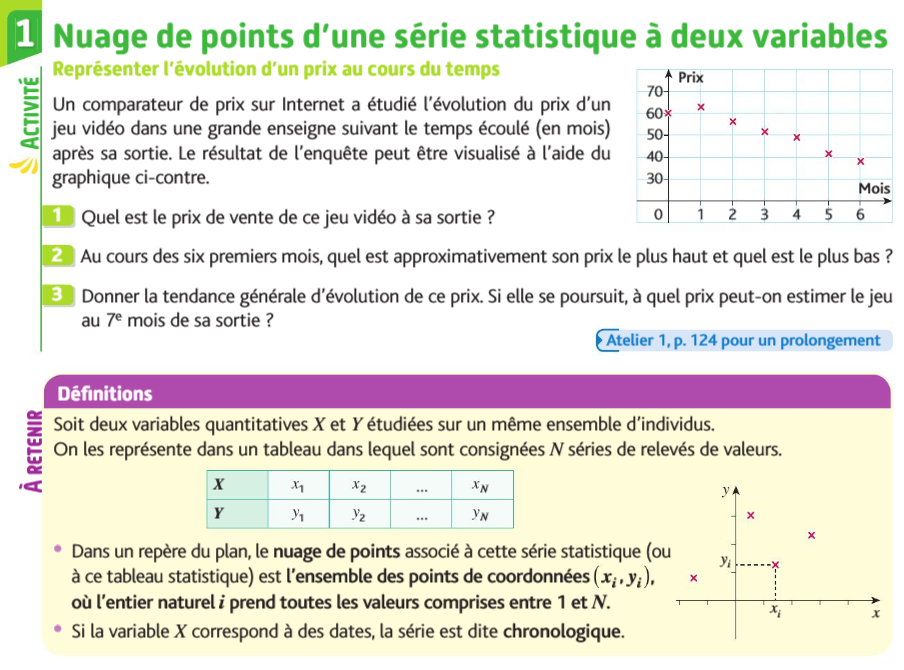
\includegraphics[width=\textwidth]{Activite.png}
\end{center}

\newpage

Le graphique suivant compare le nombre de vente en Europe et en Amérique du Nord des $100$ jeux vidéos les plus vendus en 2015.
\begin{center}
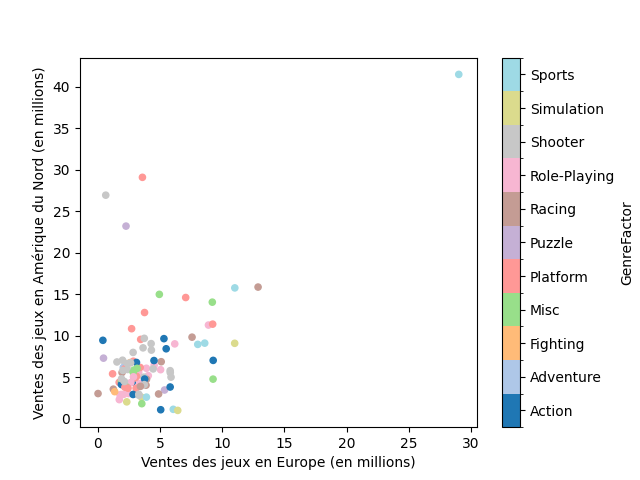
\includegraphics[width=\textwidth]{VideoGameSales.png}
\end{center}

\begin{enumerate}
\item Que représente chaque point ? Que représente les couleurs disponibles ?
\item Quel est le genre du jeu le plus vendu en 2015 ? Vous pouvez chercher le titre du jeu.
\item Quel est le genre le plus représenté ? Quel type de graphique permettrait de mieux voir cette information ?
\item La phrase \og Les jeux populaires en Europe sont tout aussi populaire en Amérique du Nord \fg vous paraît-elle vraie ? Quels jeux semblent être des contre-exemples à cette affirmation ?
\end{enumerate}

\end{document}